\begin{frame}
	\frametitle{Fitness function}
	
	\begin{columns}[c]
		
		\column{.45\textwidth}

		\begin{itemize}
			\item function for e.g. branch distance
			\item guidance for search algorithms
		\end{itemize}
		
		\begin{figure}
			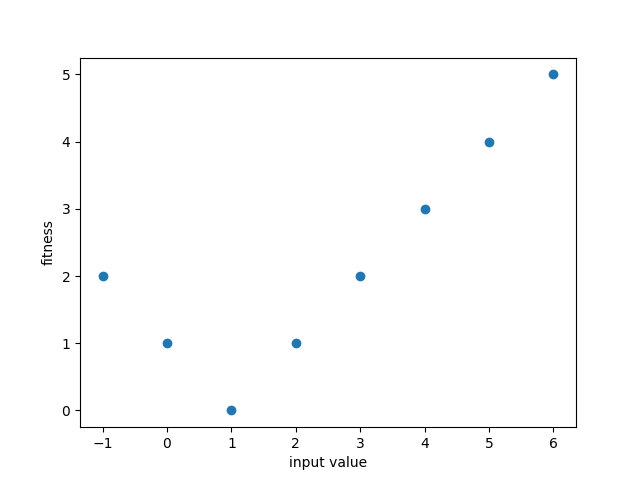
\includegraphics[width=1\textwidth]{figures/plot_guidance}
		\end{figure}
		
		\column{.45\textwidth}
		\lstinputlisting{code/simple_guidance.java}

	\end{columns}
	
\end{frame}

\begin{frame}
	\frametitle{Fitness landscape}
	
	\begin{columns}[c]
		
		\column{.45\textwidth}

		\begin{itemize}
			\item metaphor for the search space
			\item fitness value as height
			\item input as depth and width
			\item search for minima
		\end{itemize}
		
		\column{.45\textwidth}
		\begin{figure}
			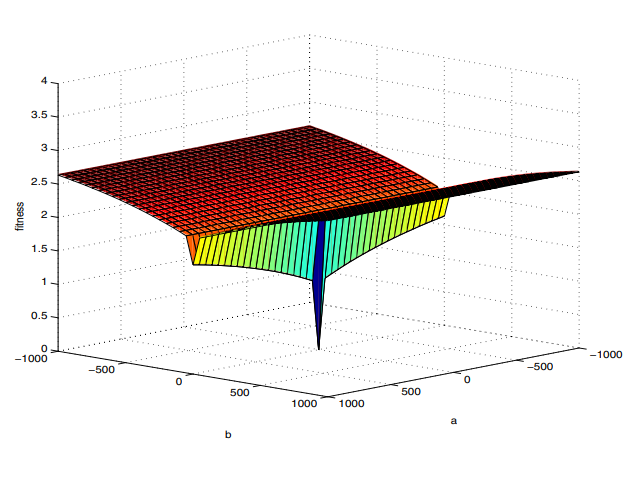
\includegraphics[width=1\textwidth]{figures/complex_landscape}
		\end{figure}
		\cite{Harman.2007}
		
	\end{columns}
	
\end{frame}

\begin{frame}
	\frametitle{Random Walk}
	\framesubtitle{\cite{Kauffman.1987}}
	
	\begin{columns}[c]
		
		\column{.45\textwidth}

		\begin{itemize}
			\item used to describe landscape
			\item walk over landscape
			\item random unbiased steps
		\end{itemize}
		
		\column{.45\textwidth}
		\begin{figure}
			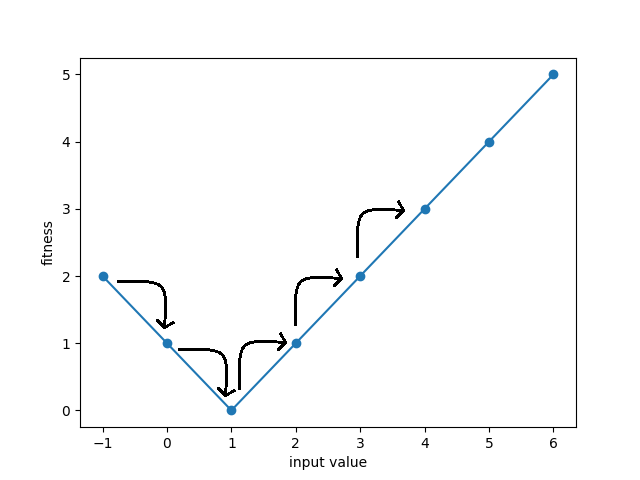
\includegraphics[width=1\textwidth]{figures/random_walk}
		\end{figure}

	\end{columns}
	
\end{frame}

\begin{frame}
	\frametitle{Long Jump}
	\framesubtitle{\cite{Kauffman.1987}}
	
	\begin{columns}[c]
		
		\column{.45\textwidth}

		\begin{itemize}
			\item multiple steps
			\item not precise 
			\item skip features (like minima)
			\item landscape approximation
		\end{itemize}
		
		\column{.45\textwidth}
		\begin{figure}
			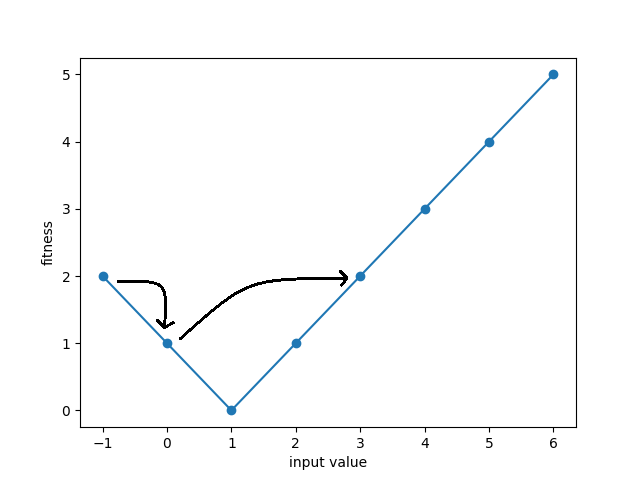
\includegraphics[width=1\textwidth]{figures/long_jump}
		\end{figure}

	\end{columns}
	
\end{frame}

\begin{frame}
	\frametitle{Genetic algorithm}
		
	\begin{itemize}
		\item unit test = individual
		\item multiple tests = population
		\item start with random population
		\item iterate till termination condition
		\begin{itemize}
			\item mutate and crossover
		\end{itemize}
		\item return last generation
	\end{itemize}
		
	
\end{frame}

\begin{frame}
	\frametitle{DynaMOSA}
	\framesubtitle{\cite{Panichella.2017}}
	
	\begin{itemize}
		\item genetic algorithm
		\item multiple target
		\item dynamic target update
		\item archive: keep track of target covering
		\item return archive as last generation individuals
		\end{itemize}
	
\end{frame}